\documentclass[a4paper, 12pt]{article}

% packages
\usepackage{amssymb}
\usepackage[fleqn]{mathtools}
\usepackage{tikz}
\usepackage{enumerate}
\usepackage{bussproofs}
\usepackage{xcolor}
\usepackage[margin=1.3cm]{geometry}
\usepackage{logicproof}
\usepackage{diagbox}
\usepackage{listings}
\usepackage{graphicx}
\usepackage{lstautogobble}
\usepackage{hyperref}
\usepackage{multirow}
\usepackage{tipa}
\usepackage{pgfplots}
\usepackage{adjustbox}

% tikz libraries
\usetikzlibrary{
    decorations.pathreplacing,
    arrows,
    shapes,
    shapes.gates.logic.US,
    circuits.logic.US,
    calc,
    automata,
    positioning,
    intersections
}

\pgfplotsset{compat=1.16}

\pgfmathdeclarefunction{gauss}{2}{%
  \pgfmathparse{1/(#2*sqrt(2*pi))*exp(-((x-#1)^2)/(2*#2^2))}%
}

\allowdisplaybreaks % allow environments to break
\setlength\parindent{0pt} % no indent

% shorthand for verbatim
% this clashes with logicproof, so maybe fix this at some point?
\catcode`~=\active
\def~#1~{\texttt{#1}}

% code listing
\lstdefinestyle{main}{
    numberstyle=\tiny,
    breaklines=true,
    showspaces=false,
    showstringspaces=false,
    tabsize=2,
    numbers=left,
    basicstyle=\ttfamily,
    columns=fixed,
    fontadjust=true,
    basewidth=0.5em,
    autogobble,
    xleftmargin=3.0ex,
    mathescape=true
}
\newcommand{\dollar}{\mbox{\textdollar}} %
\lstset{style=main}

% augmented matrix
\makeatletter
\renewcommand*\env@matrix[1][*\c@MaxMatrixCols c]{%
\hskip -\arraycolsep
\let\@ifnextchar\new@ifnextchar
\array{#1}}
\makeatother

% ceiling / floor
\DeclarePairedDelimiter{\ceil}{\lceil}{\rceil}
\DeclarePairedDelimiter{\floor}{\lfloor}{\rfloor}

% custom commands
\newcommand{\indefint}[2]{\int #1 \, \mathrm{d}#2}
\newcommand{\defint}[4]{\int_{#1}^{#2} #3 \, \mathrm{d}#4}
\newcommand{\pdif}[2]{\frac{\partial #1}{\partial #2}}
\newcommand{\dif}[2]{\frac{\mathrm{d}#1}{\mathrm{d}#2}}
\newcommand{\limit}[2]{\raisebox{0.5ex}{\scalebox{0.8}{$\displaystyle{\lim_{#1 \to #2}}$}}}
\newcommand{\limitsup}[2]{\raisebox{0.5ex}{\scalebox{0.8}{$\displaystyle{\limsup_{#1 \to #2}}$}}}
\newcommand{\summation}[2]{\sum\limits_{#1}^{#2}}
\newcommand{\product}[2]{\prod\limits_{#1}^{#2}}
\newcommand{\intbracket}[3]{\left[#3\right]_{#1}^{#2}}
\newcommand{\laplace}{\mathcal{L}}
\newcommand{\fourier}{\mathcal{F}}
\newcommand{\mat}[1]{\boldsymbol{#1}}
\renewcommand{\vec}[1]{\boldsymbol{#1}}
\newcommand{\rowt}[1]{\begin{bmatrix}
    #1
\end{bmatrix}^\top}
\DeclareMathOperator*{\argmax}{argmax}
\DeclareMathOperator*{\argmin}{argmin}

\newcommand{\lto}[0]{\leadsto\ }

\newcommand{\ulsmash}[1]{\underline{\smash{#1}}}

\newcommand{\powerset}[0]{\wp}
\renewcommand{\emptyset}[0]{\varnothing}

\makeatletter
\newsavebox{\@brx}
\newcommand{\llangle}[1][]{\savebox{\@brx}{\(\m@th{#1\langle}\)}%
  \mathopen{\copy\@brx\kern-0.5\wd\@brx\usebox{\@brx}}}
\newcommand{\rrangle}[1][]{\savebox{\@brx}{\(\m@th{#1\rangle}\)}%
  \mathclose{\copy\@brx\kern-0.5\wd\@brx\usebox{\@brx}}}
\makeatother
\newcommand{\lla}{\llangle}
\newcommand{\rra}{\rrangle}
\newcommand{\la}{\langle}
\newcommand{\ra}{\rangle}
\newcommand{\crnr}[1]{\text{\textopencorner} #1 \text{\textcorner}}
\newcommand{\bnfsep}[0]{\ |\ }
\newcommand{\concsep}[0]{\ ||\ }

\newcommand{\axiom}[1]{\AxiomC{#1}}
\newcommand{\unary}[1]{\UnaryInfC{#1}}
\newcommand{\binary}[1]{\BinaryInfC{#1}}
\newcommand{\trinary}[1]{\TrinaryInfC{#1}}
\newcommand{\quaternary}[1]{\QuaternaryInfC{#1}}
\newcommand{\quinary}[1]{\QuinaryInfC{#1}}
\newcommand{\dproof}[0]{\DisplayProof}
\newcommand{\llabel}[1]{\LeftLabel{\scriptsize #1}}
\newcommand{\rlabel}[1]{\RightLabel{\scriptsize #1}}

\newcommand{\ttbs}{\char`\\}
\newcommand{\lrbt}[0]{\ \bullet\ }

% colours
\newcommand{\violet}[1]{\textcolor{violet}{#1}}
\newcommand{\blue}[1]{\textcolor{blue}{#1}}
\newcommand{\red}[1]{\textcolor{red}{#1}}
\newcommand{\teal}[1]{\textcolor{teal}{#1}}

% reasoning proofs
\usepackage{ltablex}
\usepackage{environ}
\keepXColumns
\NewEnviron{reasoning}{
    \begin{tabularx}{\textwidth}{rlX}
        \BODY
    \end{tabularx}
}
\newcommand{\proofline}[3]{$(#1)$ & $#2$ & \hfill #3 \smallskip \\}
\newcommand{\proofarbitrary}[1]{& take arbitrary $#1$ \smallskip \\}
\newcommand{\prooftext}[1]{\multicolumn{3}{l}{#1} \smallskip \\}
\newcommand{\proofmath}[3]{$#1$ & = $#2$ & \hfill #3 \smallskip \\}
\newcommand{\prooftherefore}[1]{& $\therefore #1$ \smallskip \\}
\newcommand{\proofbc}[0]{\prooftext{\textbf{Base Case}}}
\newcommand{\proofis}[0]{\prooftext{\textbf{Inductive Step}}}

% ER diagrams
\newcommand{\nattribute}[4]{
    \node[draw, state, inner sep=0cm, minimum size=0.2cm, label=#3:{#4}] (#1) at (#2) {};
}
\newcommand{\mattribute}[4]{
    \node[draw, state, accepting, inner sep=0cm, minimum size=0.2cm, label=#3:{#4}] (#1) at (#2) {};
}
\newcommand{\dattribute}[4]{
    \node[draw, state, dashed, inner sep=0cm, minimum size=0.2cm, label=#3:{#4}] (#1) at (#2) {};
}
\newcommand{\entity}[3]{
    \node[] (#1-c) at (#2) {#3};
    \node[inner sep=0cm] (#1-l) at ($(#1-c) + (-1, 0)$) {};
    \node[inner sep=0cm] (#1-r) at ($(#1-c) + (1, 0)$) {};
    \node[inner sep=0cm] (#1-u) at ($(#1-c) + (0, 0.5)$) {};
    \node[inner sep=0cm] (#1-d) at ($(#1-c) + (0, -0.5)$) {};
    \draw
    ($(#1-c) + (-1, 0.5)$) -- ($(#1-c) + (1, 0.5)$) -- ($(#1-c) + (1, -0.5)$) -- ($(#1-c) + (-1, -0.5)$) -- cycle;
}
\newcommand{\relationship}[3]{
    \node[] (#1-c) at (#2) {#3};
    \node[inner sep=0cm] (#1-l) at ($(#1-c) + (-1, 0)$) {};
    \node[inner sep=0cm] (#1-r) at ($(#1-c) + (1, 0)$) {};
    \node[inner sep=0cm] (#1-u) at ($(#1-c) + (0, 1)$) {};
    \node[inner sep=0cm] (#1-d) at ($(#1-c) + (0, -1)$) {};
    \draw
    ($(#1-c) + (-1, 0)$) -- ($(#1-c) + (0, 1)$) -- ($(#1-c) + (1, 0)$) -- ($(#1-c) + (0, -1)$) -- cycle;
}

% AVL Trees
\newcommand{\avltri}[4]{
    \draw ($(#1)$) -- ($(#1) + #4*(0.5, -1)$) -- ($(#1) + #4*(-0.5, -1)$) -- cycle;
    \node at ($(#1) + #4*(0, -1) + (0, 0.5)$) {#3};
    \node at ($(#1) + #4*(0, -1) + (0, -0.5)$) {#2};
}

% RB Trees
\tikzset{rbtr/.style={inner sep=2pt, circle, draw=black, fill=red}}
\tikzset{rbtb/.style={inner sep=2pt, circle, draw=black, fill=black}}

% Samples
\tikzset{spos/.style={inner sep=2pt, circle, draw=black, fill=blue!20}}
\tikzset{sneg/.style={inner sep=2pt, circle, draw=black, fill=red!20}}

% Joins
\newcommand\ljoin{\stackrel{\mathclap{\normalfont\mbox{\tiny L}}}{\bowtie}}
\newcommand\rjoin{\stackrel{\mathclap{\normalfont\mbox{\tiny R}}}{\bowtie}}
\newcommand\ojoin{\stackrel{\mathclap{\normalfont\mbox{\tiny O}}}{\bowtie}}

\setcounter{MaxMatrixCols}{100}

% actual document
\begin{document}
    {\sc Computing $3^\text{rd}$ Year Notes} \hfill ~https://github.com/lin-e/imperial-revision~
    \rule{\textwidth}{0.1pt}
    \section*{CO333 - Robotics \hfill (60019)}
        \subsection*{Lecture 1 - Introduction to Robotics}
        \subsection*{Lecture 2 - Robot Motion}
            A definition of a robot is something that can \textbf{move} and \textbf{sense}, and uses some sort of information processing to link the two.
            Robots might want to move in the water, fly in the air, walk (legged) on land, or work in space.
            The course will focus on wheeled robots that work on generally flat surfaces.
            \subsubsection*{Coordinate Frames}
                \begin{center}
                    \begin{tikzpicture}
                        \node at (4, -0.5) {$x_W$};
                        \node at (-0.5, 4) {$y_W$};
                        \draw
                        (0, 0) edge[->] (4, 0)
                        (0, 0) edge[->] (0, 4)
                        (2, 0) edge[dashed] (2, 2)
                        (0, 2) edge[dashed] (2.75, 2);
                        \node[rbtb] at (2, 2) {};
                        \begin{scope}[shift={(1.8, 1.8)}]
                            \begin{scope}[rotate={45}]
                                \draw (-0.5, -0.5) -- (0.5, -0.5) -- (0.5, 0.5) -- (-0.5, 0.5) -- cycle;
                            \end{scope}
                        \end{scope}

                        \node at (3, 3.5) {$x_R$};
                        \node at (1, 3.5) {$y_R$};
                        \node at (3, 2.3) {$\theta_R$};
                        \draw
                        (2, 2) edge[->] (3, 3)
                        (2, 2) edge[->] (1, 3);
                        \draw (2, 2) ++(0:0.75) arc (0:45:0.75);
                    \end{tikzpicture}
                \end{center}
                We will be mostly focused on 2D coordinates, on the flat (close to planar) ground.
                The world frame $W$ is anchored in the world, and the robot frame $R$ is anchored to the robot (consider one point and orientation as the centre of the robot) - consider a set of axis carried by the robot.
                Often we are interested in the robot's location; the transformation between the world frame $W$ and the robot frame $R$.
            \subsubsection*{Degrees of Motion Freedom}
                This is to do with how many parameters we need to specify the aforementioned transformation, generally related to the number of dimensions the robot is moving in.
                The simplest is a single degree of freedom, where a train moves along the $x$-axis - this position can be specified in one parameter.
                A rigid body which moves on a ground plane, such as an AV or robot vacuum cleaner has 3 DoF; two translational ($x,y$) and one rotational (typically $\theta$).
                On the other hand, a rigid body which moves in 3D space has 6 degrees of freedom; three rotational and three rotational.
                \medskip

                A \textbf{holonomic robot} is able to move instantaneously in any direction in its space of DoF, otherwise it is \textbf{non-holonomic}.
                Most are non-holonomic, but some holonomic robots do exist; ground-based robots can be made with omnidirectional wheels.
                \medskip

                Standard wheel configurations (both non-holonomic; each has two motors but has three degrees of movement freedom, the number of control inputs are lower than the DoF) include;
                \begin{itemize}
                    \itemsep0em
                    \item \textbf{drive and steer} (car) - not implemented in this course
                        \smallskip

                        The combination of acceleration and braking determines how fast it moves forwards, and the orientation of wheel determines direction.
                        \begin{center}
                            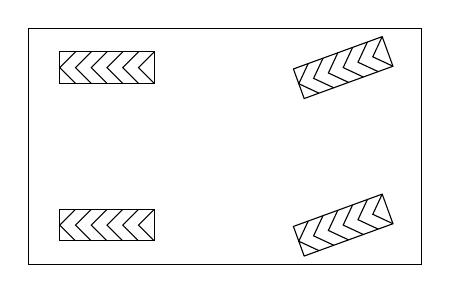
\begin{tikzpicture}
                                \draw (0, 0) -- (5, 0) -- (5, 3) -- (0, 3) -- cycle;
                                \begin{scope}[shift={(1, 2.5)}, scale={0.2}]
                                    \draw (-3, -1) -- (3, -1) -- (3, 1) -- (-3, 1) -- cycle;
                                    \foreach \i in {0,...,5} {
                                        \draw (\i - 2, 1) -- (\i - 3, 0) -- (\i - 2, -1);
                                    }
                                \end{scope}
                                \begin{scope}[shift={(1, 0.5)}, scale={0.2}]
                                    \draw (-3, -1) -- (3, -1) -- (3, 1) -- (-3, 1) -- cycle;
                                    \foreach \i in {0,...,5} {
                                        \draw (\i - 2, 1) -- (\i - 3, 0) -- (\i - 2, -1);
                                    }
                                \end{scope}
                                \begin{scope}[shift={(4, 2.5)}, rotate={20}, scale={0.2}]
                                    \draw (-3, -1) -- (3, -1) -- (3, 1) -- (-3, 1) -- cycle;
                                    \foreach \i in {0,...,5} {
                                        \draw (\i - 2, 1) -- (\i - 3, 0) -- (\i - 2, -1);
                                    }
                                \end{scope}
                                \begin{scope}[shift={(4, 0.5)}, rotate={20}, scale={0.2}]
                                    \draw (-3, -1) -- (3, -1) -- (3, 1) -- (-3, 1) -- cycle;
                                    \foreach \i in {0,...,5} {
                                        \draw (\i - 2, 1) -- (\i - 3, 0) -- (\i - 2, -1);
                                    }
                                \end{scope}
                            \end{tikzpicture}
                        \end{center}
                        Rear wheels need a differential, variable (Ackerman) linkage for steering wheels.
                    \item \textbf{differential drive} (robot vacuum)
                        \smallskip

                        Has two driving wheels, both pointing forwards, and maybe castors which keep it balanced.
                        Robot moves in different ways depending on the different speeds the wheels are turning at.
                        \begin{center}
                            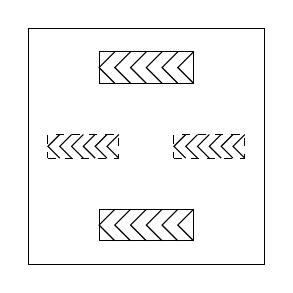
\begin{tikzpicture}
                                \draw (0, 0) -- (3, 0) -- (3, 3) -- (0, 3) -- cycle;
                                \begin{scope}[shift={(1.5, 2.5)}, scale={0.2}]
                                    \draw (-3, -1) -- (3, -1) -- (3, 1) -- (-3, 1) -- cycle;
                                    \foreach \i in {0,...,5} {
                                        \draw (\i - 2, 1) -- (\i - 3, 0) -- (\i - 2, -1);
                                    }
                                \end{scope}
                                \begin{scope}[shift={(1.5, 0.5)}, scale={0.2}]
                                    \draw (-3, -1) -- (3, -1) -- (3, 1) -- (-3, 1) -- cycle;
                                    \foreach \i in {0,...,5} {
                                        \draw (\i - 2, 1) -- (\i - 3, 0) -- (\i - 2, -1);
                                    }
                                \end{scope}
                                \begin{scope}[shift={(0.7, 1.5)}, scale={0.15}]
                                    \draw[dashed] (-3, -1) -- (3, -1) -- (3, 1) -- (-3, 1) -- cycle;
                                    \foreach \i in {0,...,5} {
                                        \draw (\i - 2, 1) -- (\i - 3, 0) -- (\i - 2, -1);
                                    }
                                \end{scope}
                                \begin{scope}[shift={(2.3, 1.5)}, scale={0.15}]
                                    \draw[dashed] (-3, -1) -- (3, -1) -- (3, 1) -- (-3, 1) -- cycle;
                                    \foreach \i in {0,...,5} {
                                        \draw (\i - 2, 1) -- (\i - 3, 0) -- (\i - 2, -1);
                                    }
                                \end{scope}
                            \end{tikzpicture}
                        \end{center}
                        The caster wheels (dashed) are passive, and simply support the robot.
                        The active wheels have one motor each.
                        If the active wheels are running at equal speeds, the robot moves in a straight line, and wheels running at equal and opposite speeds turn on the spot.
                        On the other hand, in general, other combinations lead to motion in circular arcs / curves.
                        \begin{center}
                            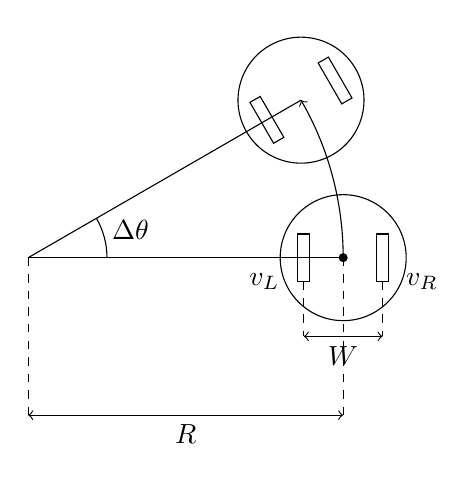
\begin{tikzpicture}
                                \begin{scope}
                                    \draw (4, 0) circle (0.8);
                                    \node[inner sep=1pt, circle, draw=black, fill=black] at (4, 0) {};
                                    \begin{scope}[shift={(3.5, 0)}, scale={0.15}]
                                        \draw (-0.5, -2) -- (-0.5, 2) -- (0.5, 2) -- (0.5, -2) -- cycle;
                                    \end{scope}
                                    \begin{scope}[shift={(4.5, 0)}, scale={0.15}]
                                        \draw (-0.5, -2) -- (-0.5, 2) -- (0.5, 2) -- (0.5, -2) -- cycle;
                                    \end{scope}
                                    \draw (0, 0) -- (4, 0);
                                \end{scope}
                                \begin{scope}[rotate={30}]
                                    \draw (4, 0) circle (0.8);
                                    \begin{scope}[shift={(3.5, 0)}, scale={0.15}]
                                        \draw (-0.5, -2) -- (-0.5, 2) -- (0.5, 2) -- (0.5, -2) -- cycle;
                                    \end{scope}
                                    \begin{scope}[shift={(4.5, 0)}, scale={0.15}]
                                        \draw (-0.5, -2) -- (-0.5, 2) -- (0.5, 2) -- (0.5, -2) -- cycle;
                                    \end{scope}
                                    \draw (0, 0) -- (4, 0);
                                \end{scope}
                                \draw (0, 0) ++(0:1) arc (0:30:1);
                                \draw[->] (0, 0) ++(0:4) arc (0:30:4);
                                \draw
                                (3.5, -1) edge[<->, below] node{$W$} (4.5, -1)
                                (0, -2) edge[<->, below] node{$R$} (4, -2);
                                \draw[dashed]
                                (0, 0) -- (0, -2)
                                (4, 0) -- (4, -2)
                                (3.5, -0.3) -- (3.5, -1)
                                (4.5, -0.3) -- (4.5, -1);
                                \node at (1.3, 0.35) {$\Delta \theta$};
                                \node at (3, -0.3) {$v_L$};
                                \node at (5, -0.3) {$v_R$};
                            \end{tikzpicture}
                        \end{center}
                        Consider the left wheel at speed $v_L$ and the right wheel at $v_R$ (linear velocities over th ground, hence $v_L = r_L\omega_L$, where $r_L$ is the radius of the wheel and $\omega_L$ is the angular velocity).
                        We also assume no slipping (the intersection is the centre of rotation).
                        \medskip

                        We want to determine $R$, which is the radius of the circle formed by the robot's centre moving.
                        Consider a small period of time $\Delta t$, and an angle of movement $\Delta \theta$;
                        $$\Delta \theta = \frac{v_L \Delta t}{R - \frac{W}{2}} = \frac{v_R \Delta t}{R + \frac{W}{2}} \Rightarrow v_L \left(R + \frac{W}{2}\right) = v_R \left(R - \frac{W}{2}\right) \Rightarrow \frac{W}{2}(v_L + v_R) = R(v_R - v_L)$$
                        By rearranging the above, and substituting back in, we have the following;
                        \begin{align*}
                            R & = \frac{W(v_R + v_L)}{2(v_R - v_L)} \\
                            \Delta \theta & = \frac{(v_R - v_L) \Delta t}{W}
                        \end{align*}
                \end{itemize}
            \subsubsection*{Actuation (DC Motors)}
                DC motors are controlled by a power signal, using \textbf{PWM (pulse width modulation)} and a fixed voltage.
                A gearing system is typically used to \textbf{gear down} the end effector to be slower with higher torque (compared to the DC motor's rapid rotation, but low torque).
                Many motors have a built in encoders (connected to the motor), which can be read to measure angular position by counting steps.
                This is required as a running motor's rotations depend on many conditions (including the load it's driving); for example a heavier robot moving on rough ground will move slower.
                To measure the rate the motor is moving at, we can feed the rotation back.
                We can then use feedback control (servo control) to adjust the motor to make it do what we want.
                In principle, we want to determine where the motor is, and where it actually is.
                At a high rate, we want to send pulses to reduce the error between the target location and actual location.
            \subsubsection*{PID (Proportional / Integral / Differential) Control}
                The PID expression sets the power as a function of error;
                $$P(t) = k_p e(t) + k_i \defint{0}{t}{e(\tau)}{\tau} + k_d \dif{e(t)}{t}$$
                In this, we have the following terms;
                \begin{itemize}
                    \itemsep0em
                    \item $e(t)$ \hfill demand minus position (error)
                        \smallskip

                        For example, at each time step this is the angle we want the motor to be at minus the actual angle of the motor measured.
                    \item $k_p$ \hfill main term (high values give rapid response)
                        \smallskip

                        Continuing with the example above, $k_p e(t)$ will be higher if $k_p$ is large.
                        If there's a large error, send a large signal, and vice versa for small errors.
                    \item $k_i$ \hfill integral term (increased to reduce steady state error)
                        \smallskip

                        Imagine the motor is close to where it should be; this allows for the `gap' to be closed.
                    \item $k_d$ \hfill differential term (reduced settling time / oscillation)
                \end{itemize}
            \subsubsection*{Wheel Rotation Speed to Velocity}
                Consider a wheel of radius $r_w$ rotating at $\omega$ (in radians per second).
                The speed of the wheel, in theory, would be $v = r_w \omega$.
                However, in practice, there are factors such as uneven ground and tyre softness, the radius may be hard to measure accurately.
                Another consideration would be possible slipping; in general it will be better to \textbf{calibrate} this for the surface by considering some constant of proportionality.
            \subsubsection*{State in 2D}
                If a robot is moving on a plane, we can define the robot with a state vector $\vec{x}$, with three parameters;
                $$\vec{x} = \begin{bmatrix}
                    x \\ y \\ \theta
                \end{bmatrix} \begin{matrix*}[l]
                    \text{$x$ component of robot centre point in world frame} \\
                    \text{$y$ component of robot centre point in world frame} \\
                    \text{rotation angle between coordinate frames (angle between $x_W$ and $x_R$ axes)}
                \end{matrix*}$$
                The two frames coincide when the robot is at the origin ($x = y = \theta = 0$).
                Note that $-\pi < \theta \leq \pi$.
                During a straight line period of motion of distance $D$, we have;
                $$\begin{bmatrix}
                    x^\prime \\
                    y^\prime \\
                    \theta^\prime
                \end{bmatrix} = \begin{bmatrix}
                    x + D \cos \theta \\
                    y + D \sin \theta \\
                    \theta
                \end{bmatrix}$$
                On the other hand, during a pure rotation of angle $\alpha$ we have (rotation to the left is positive by convention);
                $$\begin{bmatrix}
                    x^\prime \\
                    y^\prime \\
                    \theta^\prime
                \end{bmatrix} = \begin{bmatrix}
                    x \\
                    y \\
                    \theta + \alpha
                \end{bmatrix}$$
        \subsection*{Lecture 3 - Sensors (Behaviours)}
            \subsubsection*{Motivation}
                Recall the second practical; there was a gradual drift from the desired path.
                There are aspects of the world that the robot can never fully understand (such as the bumpiness of the floor) - even simulations cannot do exactly the same thing every time.
                After calibration, the robot should return to the desired location (on average), but some scatter will remain due to factors we cannot control.
                \medskip

                Systematic errors are removed, however we still have \textbf{zero mean errors} - these errors occur incrementally (where every movement or rotation adds a small amount of potential error).
                The zero mean errors can be modelled probabilistically, often with a Gaussian distribution.
            \subsubsection*{Uncertainty in Motion}
                A better model (compared to the previous lecture) adds uncertain perturbations / motion noise;
                $$\begin{bmatrix}
                    x^\prime \\
                    y^\prime \\
                    \theta^\prime
                \end{bmatrix} = \begin{bmatrix}
                    x + (D + e) \cos \theta \\
                    y + (D + e) \sin \theta \\
                    \theta + f
                \end{bmatrix}$$
                We will likely also notice that rotations are not exact either;
                $$\begin{bmatrix}
                    x^\prime \\
                    y^\prime \\
                    \theta^\prime
                \end{bmatrix} = \begin{bmatrix}
                    x \\
                    y \\
                    \theta + \alpha + g
                \end{bmatrix}$$
            \subsubsection*{Sensors}
                Proprioceptive are self-sensing (such as motor encoders / internal force sensors) and improve a robot's sense of its own internal state.
                In general, these measurements may depend on the previous states as (as well as the current state); for example wheel odometry gives a reading depending on a difference between the current and previous state, on the other hand, a gyro in an inertial measurement unit will report a reading depending on the current \textbf{rate} of rotation (not an instantaneous state).
                \medskip

                In this case, the value of the measurement $\vec{z}_p$ should be a function of the state of the state of the robot;
                $$\vec{z}_p = \vec{z}_p(\vec{x})$$

                On the other hand, exteroceptive are outward-looking.
                These allow the robot to generally be \textbf{aware} of its environment, letting it localise with respect to a map, recognise objects / locations, map out free space, avoid obstacles, and interact with objects.
                \medskip

                In this case, we need both the sate of the robot $\vec{x}$ and the state of the world $\vec{y}$ (relative to the robot);
                $$\vec{z}_o = \vec{z}_o(\vec{x}, \vec{y})$$
                The state of the world may be parameterised (such as a list of geometric coordinates describing landmarks).
                This state may be uncertain.
                \medskip

                Some sensors (such as touch, light, and sonar) will return a \textbf{single value} in a range.
                On the other hand, some sensors such as a camera or laser range-finder will return an \textbf{array} of values, with the former having an array of sensing elements (pixels of a camera's CCD chip), or the latter performing scanning.
                \medskip

                Some common sensors are as follows;
                \begin{itemize}
                    \itemsep0em
                    \item \textbf{touch sensor}
                        \smallskip

                        This is a binary on / off state; an open switch will have no current flow, and a closed switch will have current flow (hit).
                    \item \textbf{light sensor}
                        \smallskip

                        This detects intensity of passive light incident from a single forward direction (some range of angle sensitivity); this is a continuous value.
                        Multiple sensors can guide steering behaviours (such as driving towards a brighter light).
                        In \textit{Lego}, there is also a mode where the sensor can emit light, where reflections from close surfaces can be measured.
                    \item \textbf{sonar (ultrasonic) sensors}
                        \smallskip

                        Sonar measures distance by emitting ultrasonic pulses (tiny pulses of sound at a high frequency) - these beams typically have an angular width of $10^\circ - 20^\circ$.
                        The sensors measure the time for a pulse to bounce back (which the sensor uses to calculate the distance).
                        These are fairly accurate within a few centimetres in one direction (for simple shapes) - but can be noisy in the presence of complicated shapes.
                        The maximum range is a few metres.
                    \item \textbf{laser range-finder}
                        \smallskip

                        The principle of this is similar to sonar, however it uses infrared laser beams instead of sound.
                        This is also reflected, detected, and timed to calculate a distance.
                        These are very accurate (sub-millimetre), and work on most surfaces.
                        They can normally scan in a 2D plane (rotating on one axis), but can also scan in 3D.
                        Previously, these were bulky and expensive, however nowadays they are present in modern smartphones.
                \end{itemize}
            \subsubsection*{Vision}
                This is the generalisation of a light sensor.
                A camera can be thought of as a large array of light sensors (or a light sensor is a single pixel of) which returns a large, rectangular array of measurements.
                A single camera measures light intensity (rather than direct information about geometry).
            \subsubsection*{Bump Detection (Touch Sensor)}
                We can either perform this with a touch sensor, or by thresholding sonar (such as if the distance falls below some range).
                \medskip

                Multiple touch sensors mounted inside a floating skirt can allow for detection of where an obstacle was hit.
                For example, if a robot was hit at the front, it may attempt to drive around it by going backwards, moving around, and continuing.
                Another simple strategy is to rotate through a random angle and go forward until the next collision (random bounce).
            \subsubsection*{Servoing}
                Servoing is a control technique where control parameters (e.g. the desired speed of a motor) are coupled directly to a sensor reading and updated regularly in a \textbf{negative feedback loop} - this is also known as \textbf{closed loop control}.
                This requires high frequency updates of both the sensor and the update, otherwise the motion can oscillate.
                \medskip

                Propeortional control sets the demand proportional to negative error - for example in velocity (where we look at the difference between the desired sensor value and actual sensor value);
                $$v = -k_p (z_\text{desired} - z_\text{actual})$$
                This proportional case is a specific case of PID control.
                \medskip

                A simple steering law to guide the robot to collide with the target would be as follows (for example - if the obstacle is straight ahead ($\alpha = 0$), then don't steer);
                $$s = k_p \alpha$$
                On the other hand, to guide the robot to avoid the obstacle at a safe distance ($R$) would subtract an offset ($D$ is the distance from the robot to the object, and $\alpha$ is the angle between the robot's rotation and the direction to the object);
                $$s = k_p(\alpha - \sin^{-1}\frac{R}{D})$$
            \subsubsection*{Wall Following}
                Consider the following scenario, where a differential drive robot desires to travel along a wall, at some distance $d$.
                This uses a \textbf{sideways-looking sonar} to measure some distance $z$.
                In the following diagram, the wall can be curved; I just don't know how to do that in TikZ.
                \begin{center}
                    \begin{tikzpicture}
                        \draw (-3, 3) -- (10, 3);
                        \begin{scope}[scale={0.5}]
                            \draw (0, 0) -- (3, 0) -- (3, 3) -- (0, 3) -- cycle;
                            \begin{scope}[shift={(1.5, 2.5)}, scale={-0.2}]
                                \draw (-3, -1) -- (3, -1) -- (3, 1) -- (-3, 1) -- cycle;
                                \foreach \i in {0,...,5} {
                                    \draw (\i - 2, 1) -- (\i - 3, 0) -- (\i - 2, -1);
                                }
                            \end{scope}
                            \begin{scope}[shift={(1.5, 0.5)}, scale={-0.2}]
                                \draw (-3, -1) -- (3, -1) -- (3, 1) -- (-3, 1) -- cycle;
                                \foreach \i in {0,...,5} {
                                    \draw (\i - 2, 1) -- (\i - 3, 0) -- (\i - 2, -1);
                                }
                            \end{scope}
                            \begin{scope}[shift={(0.7, 1.5)}, scale={-0.15}]
                                \draw[dashed] (-3, -1) -- (3, -1) -- (3, 1) -- (-3, 1) -- cycle;
                                \foreach \i in {0,...,5} {
                                    \draw (\i - 2, 1) -- (\i - 3, 0) -- (\i - 2, -1);
                                }
                            \end{scope}
                            \begin{scope}[shift={(2.3, 1.5)}, scale={-0.15}]
                                \draw[dashed] (-3, -1) -- (3, -1) -- (3, 1) -- (-3, 1) -- cycle;
                                \foreach \i in {0,...,5} {
                                    \draw (\i - 2, 1) -- (\i - 3, 0) -- (\i - 2, -1);
                                }
                            \end{scope}
                        \end{scope}
                        \draw (0.75, 0.75) edge[->, right] node{$v$} (0.75, 3);
                        \draw (-0.1, 1.5) edge[<->, left] node{$d$} (-0.1, 3);
                    \end{tikzpicture}
                \end{center}
                Note that we are moving left to right (along the diagram), and we want to steer towards the wall (since we'd ideally have $d = v$).
                To do this, the left wheel must turn slower than the right wheel.
                Note that we can also achieve symmetric behaviour with a constant offset $v_C$ (standard speed for a straight line).
                We can then set the left and right wheel velocities as follows;
                \begin{align*}
                    v_R - v_L & = k_p(z - d) \\
                    v_R & = v_C + \frac{1}{2}k_p(z - d) \\
                    v_L & = v_C - \frac{1}{2}k_p(z - d)
                \end{align*}
            \subsubsection*{Combining}
                More complex robots may have multiple servos, and we can combine sensing-action loops.
                We can instead consider each local servo-like sensing-action loop as a \textbf{behaviour}.
                These behaviours can then be combined in an \textbf{arbiter}, which feeds the instructions into a motor controller.
                \medskip

                To go further, we need to go beyond a coupling between sensors and actions, and instead build a model of the world.
                Here we plan a sequence of actions to achieve a goal, and then execute the plan.
                However, if the world changes during the execution, we need to re-plan the actions.
        \subsection*{Lecture 4 - Probabilistic Robotics}
            From the previous lab, we notice an issue when the robot is at a large angle to the wall; we realistically want the perpendicular distance between the robot and the wall, but this gets much larger if the robot is at a large angle.
            One solution is to mount the camera in front of the robot, as this couples rotation with distance.
            \subsubsection*{Probabilistic Localisation}
                Notice from the previous labs that attempting to estimate the location of the robot can lead to errors adding up.
                We assume some knowledge of the scene, but we do not know the location of the robot relative to the map.
                Long-term estimation based on logical reasoning fail when presented with real data; advanced sensors cannot be easily analysed like bump and light sensors, and all information received is uncertain (every action as well as every sensor measurement).
                A probabilistic robot acknowledges the uncertainty (and uses models to abstract useful information).
                \begin{center}
                    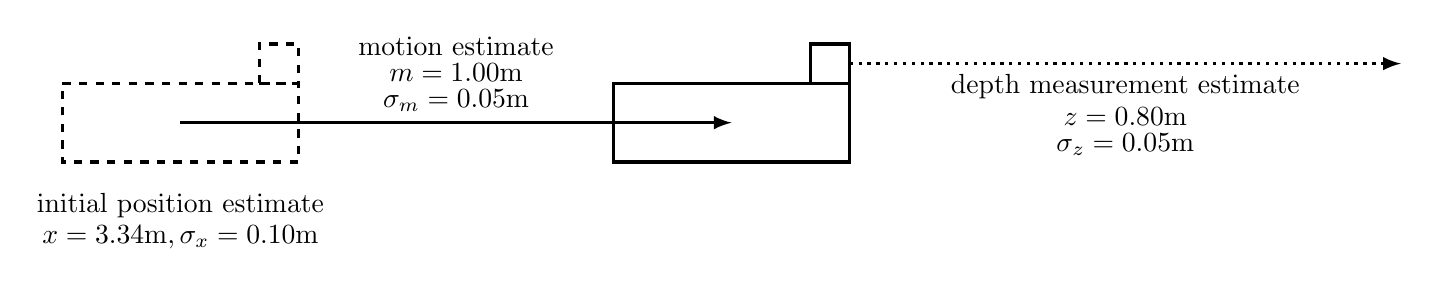
\begin{tikzpicture}
                        \begin{scope}
                            \draw[very thick, dashed]
                            (0, 0) -- (3, 0) -- (3, -1) -- (0, -1) -- cycle
                            (2.5, 0) -- (3, 0) -- (3, 0.5) -- (2.5, 0.5) -- cycle;
                        \end{scope}
                        \draw (1.5, -0.5) edge[-latex, very thick, above] node{\shortstack{motion estimate\\$m = 1.00\mathrm{m}$\\$\sigma_m = 0.05\mathrm{m}$}} (8.5, -0.5);
                        \begin{scope}[shift={(7, 0)}]
                            \draw[very thick]
                            (0, 0) -- (3, 0) -- (3, -1) -- (0, -1) -- cycle
                            (2.5, 0) -- (3, 0) -- (3, 0.5) -- (2.5, 0.5) -- cycle;
                        \end{scope}
                        \node at (1.5, -1.75) {\shortstack{initial position estimate\\$x = 3.34\mathrm{m}, \sigma_x = 0.10\mathrm{m}$}};
                        \draw (10, 0.25) edge[-latex, dotted, very thick, below] node{\shortstack{depth measurement estimate\\$z = 0.80\mathrm{m}$\\$\sigma_z = 0.05\mathrm{m}$}} (17, 0.25);
                    \end{tikzpicture}
                \end{center}
                When we start with an uncertain position, and make an uncertain motion, the robot will have an uncertain state measurement.
                Once the robot then performs some measurement, there will likely be some uncertainty in the result.
            \subsubsection*{Probabilistic Inference}
                We think of what we want to estimate, and then their probabilistic relation to things we can actually observe.
                The following graph is one visualisation of a SLAM problem;
                \begin{center}
                    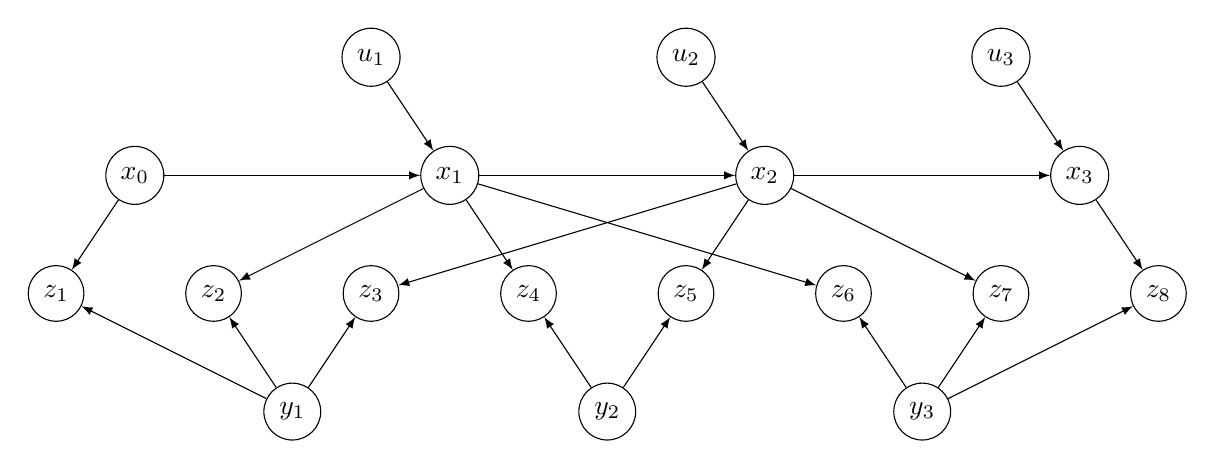
\begin{tikzpicture}[y=0.75cm]
                        \node[draw, circle] (x0) at (0, 0) {$x_0$};
                        \node[draw, circle] (x1) at (4, 0) {$x_1$};
                        \node[draw, circle] (x2) at (8, 0) {$x_2$};
                        \node[draw, circle] (x3) at (12, 0) {$x_3$};
                        \node[draw, circle] (u1) at (3, 2) {$u_1$};
                        \node[draw, circle] (u2) at (7, 2) {$u_2$};
                        \node[draw, circle] (u3) at (11, 2) {$u_3$};
                        \node[draw, circle] (z1) at (-1, -2) {$z_1$};
                        \node[draw, circle] (z2) at (1, -2) {$z_2$};
                        \node[draw, circle] (z3) at (3, -2) {$z_3$};
                        \node[draw, circle] (z4) at (5, -2) {$z_4$};
                        \node[draw, circle] (z5) at (7, -2) {$z_5$};
                        \node[draw, circle] (z6) at (9, -2) {$z_6$};
                        \node[draw, circle] (z7) at (11, -2) {$z_7$};
                        \node[draw, circle] (z8) at (13, -2) {$z_8$};
                        \node[draw, circle] (y1) at (2, -4) {$y_1$};
                        \node[draw, circle] (y2) at (6, -4) {$y_2$};
                        \node[draw, circle] (y3) at (10, -4) {$y_3$};

                        \draw
                        (u1) edge[-latex] (x1)
                        (u2) edge[-latex] (x2)
                        (u3) edge[-latex] (x3)
                        (x0) edge[-latex] (x1)
                        (x1) edge[-latex] (x2)
                        (x2) edge[-latex] (x3)
                        (x0) edge[-latex] (z1)
                        (x1) edge[-latex] (z2)
                        (x1) edge[-latex] (z4)
                        (x1) edge[-latex] (z6)
                        (x2) edge[-latex] (z3)
                        (x2) edge[-latex] (z5)
                        (x2) edge[-latex] (z7)
                        (x3) edge[-latex] (z8)
                        (y1) edge[-latex] (z1)
                        (y1) edge[-latex] (z2)
                        (y1) edge[-latex] (z3)
                        (y2) edge[-latex] (z4)
                        (y2) edge[-latex] (z5)
                        (y3) edge[-latex] (z6)
                        (y3) edge[-latex] (z7)
                        (y3) edge[-latex] (z8);
                    \end{tikzpicture}
                \end{center}
                Note that in the above diagram, the nodes $x_i$ denote the estimate of the location of the robot at some point in time.
                We are also interested in estimating the locations of landmarks in the world (denoted by $y_i$ - fixed landmarks).
                The sensors (such as camera or sonar) will make some sort of measurement relative to the position robot ($z_i$) - for example, at $x_1$ the robot observes $y_1, y_2, y_3$ with measurements $x_2, z_4, z_6$ respectively.
                Finally, the control inputs (for the movement) are denoted by $u_i$.
                \medskip

                The process of \textbf{sensor fusion} combines data from many different sources to create useful estimates.
                This state estimate can be used to decide the next action.
                \medskip

                Probabilities describe our state of knowledge (not randomness, which is rare in the real world).
                For example, the physics for a coin flip are deterministic, however without this knowledge, we can only guess the outcome.
                % We are using it (Bayesian viewpoint) as a tool to reason 
                $$P(XZ) = P(Z\ |\ X)P(X) = P(X\ |\ Z)P(X) \Rightarrow \underbrace{P(X\ |\ Z)}_{(1)} = \frac{\overbrace{P(Z\ |\ X)}^{(2)}\overbrace{P(X)}^{(3)}}{\underbrace{P(Z)}_{(4)}}$$
                \begin{enumerate}[(1)]
                    \itemsep0em
                    \item posterior
                    \item likelihood
                    \item prior
                    \item marginal likelihood
                \end{enumerate}
                In the state diagram, we have things we are interested in estimating (state variables) and things we can get from sensors (measurements / observations).
                Typically state variables are represented with $X$ in the probabilities, with measurements being represented by $Z$.
                Bayes' rule is used to incrementally digest new information; we have a prior estimate of $X$ already - $P(X)$.
                From this, we want to get the probability of $X$ given $Z$ - $P(X\ |\ Z)$.
                We want to obtain $P(Z\ |\ X)$, which is the likelihood of the measurement given the state variable.
                \medskip

                Consider the following example;
                \begin{center}
                    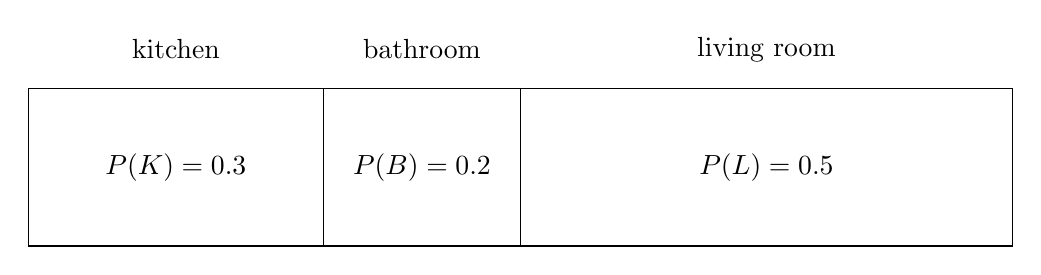
\begin{tikzpicture}[x=1.25cm]
                        \draw
                        (0, 0) -- (10, 0) -- (10, -2) -- (0, -2) -- cycle
                        (3, 0) -- (3, -2)
                        (5, 0) -- (5, -2);
                        \node at (1.5, 0.5) {kitchen};
                        \node at (1.5, -1) {$P(K) = 0.3$};
                        \node at (4, 0.5) {bathroom};
                        \node at (4, -1) {$P(B) = 0.2$};
                        \node at (7.5, 0.5) {living room};
                        \node at (7.5, -1) {$P(L) = 0.5$};
                    \end{tikzpicture}
                \end{center}
                The robot starts completely lost, let the probability of it being in each room be proportional to the area (note that the probabilities are normalised).
                Assume we also have some light sensor (which gives a thresholded value of it either being light or dark), which has had experiments performed in each of the rooms to obtain probabilities.
                Assume the sensor also now reports it as being bright (hence we want to find the probability of it being in a room, \textbf{given} that it is bright).
                \begin{align*}
                    P(b\ |\ K) & = 0.8 & \text{bright 80\% of the time in the kitchen} \\
                    P(K\ |\ b) & = \frac{P(K)P(b\ |\ K)}{P(b)} \\
                    & = \frac{0.3 \times 0.8}{P(b)} \\
                    & = \frac{0.24}{P(b)} \\
                    & = 0.4 \\
                    P(b\ |\ B) & = 0.3 & \text{bright 30\% of the time in the bathroom} \\
                    P(B\ |\ b) & = \frac{P(B)P(b\ |\ B)}{P(b)} \\
                    & = \frac{0.2 \times 0.3}{P(b)} \\
                    & = \frac{0.06}{P(b)} \\
                    & = 0.1 \\
                    P(b\ |\ L) & = 0.6 & \text{bright 60\% of the time in the living room} \\
                    P(L\ |\ b) & = \frac{P(L)P(b\ |\ L)}{P(b)} \\
                    & = \frac{0.5 \times 0.6}{P(b)} \\
                    & = \frac{0.3}{P(b)} \\
                    & = 0.5
                \end{align*}
                However, note that the sum of the posteriors must also be equal to 1, hence;
                $$P(K\ |\ b) + P(B\ |\ b) + P(L\ |\ b) = 1 \Rightarrow \frac{0.24 + 0.06 + 0.3}{P(b)} = 1 \Rightarrow P(b) = 0.6$$
                Note that in the example above, we've digested information that suggests the robot being in the kitchen (due to the brightness), hence the probability of it being in the kitchen has gone up, whereas the probability of it being located in the bathroom has gone down.
            \subsubsection*{Probability Distribution}
                Discrete inference generalises to more possible states as the bins get smaller and smaller (for example, if we were to divide the floorplan into more zones).
                As the width of the bins tend to 0, we have a continuous probability density function $p(x)$ at the limit.
                The probability that a continuous parameter lies in the range $a$ to $b$ is;
                $$P_{a \to b} \defint{a}{b}{p(x)}{x}$$
                However, as the resolution becomes higher, it is becomes more expensive in terms of memory and computation.
                \medskip

                Gaussian distributions often represent the uncertainty in sensor measurements well, parametising a 1D distribution in two parameters ($\mu$ and $\sigma$);
                $$p(x) = \frac{1}{\sqrt{2 \pi}\sigma} e^{-\frac{(x - \mu)^2}{2 \sigma^2}}$$
                A Gaussian prior multiplied by a likelihood will produce a posterior tighter than both.
                The product of two Gaussians is \textbf{always} another Gaussian.
                However, there is only one peak, which may not always fit.
            \subsubsection*{Particle Filtering}
                Another representation is to use particles.
                A probability distribution here is represented with a finite set of weighted samples (typically $N = 100$) of the state;
                $$\{ \vec{x_i}, w_i \} = \left\{\begin{bmatrix}
                    x_i \\ y_i \\ \theta_i
                \end{bmatrix}, w_i\right\}\text{ where } \summation{i=1}{N}w_i = 1$$
                Instead of storing a large table of numbers, we almost entirely ignore where the probability is low (close to 0), and focus on the areas where there is higher probability.
                We want to store the probability distribution within the degrees of freedom of the robot.
                The idea here is to test the hypothesis of where the robot is (the cloud of points) and narrow it down based on sensor observations - a good estimate is a tight clump of particles.
                \medskip

                In general, these steps are repeated every time the robot moves and makes measurements;
                \begin{enumerate}[1.]
                    \itemsep0em
                    \item motion prediction based on \textbf{proprioceptive} sensors
                        \smallskip

                        With blind motion, the particles should spread out more and more (due to a growing uncertainty).
                        For this, we use the state changes with the zero mean noise terms ($e, f, g$) - these are generated randomly for \textbf{each} particle.
                        \medskip

                        Also note that the robot may move through variable step sizes, and we will need to scale the variance accordingly.
                    \item measurement update based on outward-looking sensors
                    \item normalisation
                    \item resampling
                        \smallskip

                        Redistributes positions of particles - particles will spread out under motion, but will acquire different weights based on how well they agree with the sensor measurements, according to Bayes' rule (higher weights for more probable locations).
                \end{enumerate}
                At any point in time, our uncertain estimate of the location of the robot is represented by the whole particle set; we can make a point estimate of the current state by taking the (weighted) mean of the particles;
                $$\vec{\bar{x}} = \summation{i = 1}{N} w_i\vec{x_i}$$
                This state can be used to plan waypoint navigation.
            \subsubsection*{Position-Based Path Planning}
                Assume the current state of the robot is $(x, y, \theta)$, and we want to travel to a waypoint set at $(W_x, W_y)$.
                We need to first rotate towards the waypoint, with the following direction vector;
                $$\begin{bmatrix}
                    d_x \\ d_y
                \end{bmatrix} = \begin{bmatrix}
                    W_x - x \\
                    W_y - y
                \end{bmatrix}$$
                This can be used to obtain an \textbf{absolute} angular orientation $\alpha$, which the robot must drive in;
                $$\alpha = \tan^{-1}\frac{d_y}{d_x}$$
                We need to make sure that $\alpha$ is in the correct quadrant of $(-\pi, pi]$, as a standard $\tan^{-1}$ function would give a value in the range $(-\frac{\pi}{2}, \frac{\pi}{2}]$.
                This can also be achieved with ~atan2(dy, dx)~ in many languages.
                \medskip

                Using this, we can obtain the angle the robot must rotate through as $\beta$ (and we should take care to shift this angle into the range $(-\pi, \pi]$ for efficient movement).
                The robot should then drive through a distance $d$ in a straight line;
                \begin{align*}
                    \beta & = \alpha - \theta \\
                    d & = \sqrt{d_x^2 + d_y^2}
                \end{align*}
        \subsection*{Lecture 5 - Monte Carlo Localisation}
            In this practical, we aim to perform localisation within a map (which is known by the robot in advance).
            \begin{center}
                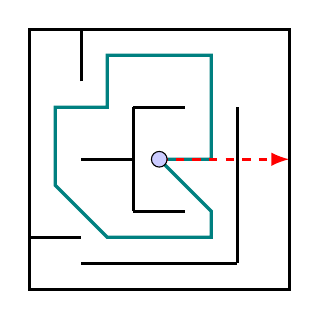
\begin{tikzpicture}[x=0.33cm, y=0.33cm]
                    \draw[very thick, teal]
                    (5, 5) -- (7, 5) -- (7, 9) -- (3, 9) -- (3, 7) -- (1, 7) -- (1, 4) -- (3, 2) -- (7, 2) -- (7, 3) -- cycle;

                    \draw[very thick, red] (5, 5) edge[-latex, dashed] (10, 5);
                    \node[spos] at (5, 5) {};

                    \draw[very thick]
                    (0, 0) -- (10, 0) -- (10, 10) -- (0, 10) -- cycle
                    (2, 1) -- (8, 1)
                    (8, 1) -- (8, 7)
                    (0, 2) -- (2, 2)
                    (4, 3) -- (6, 3)
                    (4, 3) -- (4, 7)
                    (2, 5) -- (4, 5)
                    (4, 7) -- (6, 7)
                    (2, 8) -- (2, 10);
                \end{tikzpicture}
            \end{center}
            MCL uses a cloud of weighted particles to represent the uncertain position, and can be thought of in two ways;
            \begin{itemize}
                \itemsep0em
                \item a Bayesian probabilistic filter
                \item similar to a genetic algorithm (survival of the fittest)
                    \smallskip

                    Each particle is a hypothesis, and we can test whether this is sensible or not by using the new measurement from the sonar.
                    The particles are then assigned a fitness, either increased if they agree with the measurement, and decreased if not.
                    The fitter particles will make more copies of themselves in the resampling stage (leading to the unfit ones dying out).
            \end{itemize}
            Note that with the weighted particle distribution, we can interpret it as a probability that the robot is within any multi-dimensional region of the state space being the sum of the weights within that region.
            However, this could break if we select a very small region between particles - but this is a trade-off we make for performance.
            \medskip

            MCL targets both of the following problems;
            \begin{itemize}
                \itemsep0em
                \item \textbf{continuous localisation}
                    \smallskip

                    This is a tracking problem, where we want to estimate the robot's new position given the an estimate of its location in the last time-step.
                    If we assume that we start at a perfectly known location, we can set the state of all particles to be the exact same.
                    The weights would all be equal to $\frac{1}{N}$, and we have a spike representing the robot's location.
                \item \textbf{global localisation}
                    \smallskip

                    In contrast, we only know the robot is within a certain region (somewhere within a room).
                    Particles can be initialised to be random positions and orientations within the room, the weights are also all equal again.
                    This is difficult with a single sensor
            \end{itemize}
            Our estimate of the robot's location is represented by th particle set, and we can get a point estimate of the current state by taking the mean of all the particles (if the weights weren't equal, it would be more biased towards the higher weights);
            $$\bar{\vec{x}} = \summation{i=1}{N}w_i\vec{x_i}$$
            \subsubsection*{Measurement Updates}
                An update consists of applying Bayes Rule to each particle.
                When we have a measurement $z$, the weights are updated as follows (the denominator in Bayes' rule is a constant that will be removed by normalisation, hence we ignore it);
                $$w_{i (new)} = \violet{P(z\ |\ \vec{x_i})} \cdot w_i$$
                The \violet{likelihood} of particle $i$ is the probability of getting the measurement $z$ given that $\vec{x_i}$ represents the true state.
            \subsubsection*{Likelihood Functions}
                A likelihood function fully describes the sensor's performance.
                This function has two inputs; the measurement we've achieved ($z$) and the state variables (ground truth) $v$.
                If there is no systematic error, and the uncertainty is constant, we would have multiple Gaussian distributions (assuming the sensor can be modelled as such) along the line $z = v$.
                This is slightly difficult to visualise, but consider a Gaussian hill (multiple distributions).
                If we took one slice (a specific $v$) value, we'd have a distribution with the mean at $v$.
                \medskip

                Different sensors will have different characteristics.
                A sonar typically doesn't have much variation no matter the distance (when plotted, the shape stays the same and only the mean changes), whereas other sensors such as stereo vision camera system will have less accuracy the further away it is (hence the Gaussian becomes flatter as $v$ increases, representing larger spread).
            \subsubsection*{Obtaining Ground Truth}
                We can obtain the ground truth as follows;
                \begin{center}
                    \begin{tikzpicture}
                        \node[rbtb] (r) at (0, 0) {};
                        \node[rbtb] (a) at (2, 3.33) {};
                        \node[rbtb] (b) at (6, 2) {};
                        \draw
                        (0, 0) -- (1.25, 0)
                        (a) -- (b)
                        (0, 0) edge[-latex, above] node{$m$} (4.8, 2.4)
                        (0, 0) ++(0:1) arc (0:26.6:1);

                        \node at ($(a) + (-1, 0)$) {$(A_x, A_y)$};
                        \node at ($(b) + (1, 0)$) {$(B_x, B_y)$};
                        \node at ($(r) + (0, -0.5)$) {robot at $(x, y, \theta)$};
                        \node at (1.25, 0.25) {$\theta$};
                    \end{tikzpicture}
                \end{center}
                Note that $m$ is the forward distance (at angle $\theta$) to an \textbf{infinite wall} passing through the points $\vec{A}$ and $\vec{B}$;
                $$m = \frac{(B_y - A_y)(A_x - x) - (B_x - A_x)(A_y - y)}{(B_y - A_y)\cos \theta - (B_x - A_x)\sin \theta}$$
                \medskip

                For each wall, we work out the value $m$.
                One criteria is that the $m$ must be positive (since the sonar would give a positive measurement).
                Furthermore, we also need to check if the point it intersects is actually between the endpoints of the wall (since the walls are considered to be infinite).
                Additionally, if several points are valid, the closest one is the one it is actually responding to.
                The point on the wall can be calculated as;
                $$\begin{bmatrix}
                    x + m\cos(\theta) \\
                    y + m\sin(\theta)
                \end{bmatrix}$$
            \subsubsection*{Likelihood}
                The likelihood should depend on the difference $z - m$; if this is small then it validates a particle (and weakens the particle if large).
                A Gaussian function is usually a good model for the mathematical form for this, with the standard deviation $\sigma_s$ being based on our model of how uncertain the sensor is (and may either be constant or depend on $z$).
                $$p(z\ |\ m) \propto e^{-\frac{(z - m)^2}{2\sigma_s^2}} \violet{+ K}$$ % check this
                We may consider modifying the Gaussian distribution to make the likelihood function more \textbf{robust}.
                This is more applicable in real-world robotics (which may give garbage data, possibly due to poor electronics etc.).
                A Gaussian normally states that there is almost no chance of it getting a value very far from the mean, however by \textbf{adding a constant}, it creates a \textbf{heavy tail}, which gives a constant probability the sensor may report garbage data, uniformly distributed across the range of the sensor.
                \medskip

                In MCL, this causes the filter to be less aggressive in removing particles which are far from agreeing with a measurement.
                This prevents a garbage measurement killing off particles in good positions.
                \medskip

                Another factor we may want to consider is the angle between the sonar direction and the normal to the wall, $\beta$.
                If this is too large, the sonar reading may not be sensible.
                $$\beta = \cos^{-1}\left(\frac{\cos \theta (A_y - B_y) + \sin \theta (B_x - A_x)}{\sqrt{(A_y - B_y)^2 + (B_x - A_x)^2}}\right)$$
            \subsubsection*{Resampling}
                All the weights should now be scaled to add up to 1;
                $$w_{i(new)} = \frac{w_i}{\summation{i=1}{N} w_i}$$
                Resampling involves generating the new set of $N$ particles, each having equal weights, but with a spatial distribution reflecting the probability density.
                To do this, we copy the state of one of the previous particles with the probability according to the particle's weight.
                This can be achieved by generating the cumulative probability distribution of the particles and generating a random number (between 0 and 1 if normalised), and picking the particle that this random number intersects.
                It's possible to skip the normalisation step and resample from an unnormalised distribution in a similar way (for efficiency).
            \subsubsection*{Compass Sensor}
                This process is quite general, and can also be done with other sensors.
                Consider a compass that measures the bearing $\beta$ relative to magnetic north.
                The likelihood $P(\beta\ |\ \vec{x_i})$ only depends on the $\theta$ component of $\vec{x_i}$.
                If the compass is working perfectly, then we have the following (where $\gamma$ denotes the magnetic bearing of the $x$ coordinate axis of frame $W$);
                $$\beta = \gamma - \theta$$
                The likelihood then depends on the difference between $\beta$ and $\gamma - \theta$;
                $$e^{-\frac{(\beta - (\gamma - \theta))^2}{2\sigma_c^2}}$$
        \subsection*{Lecture 6 - Advanced Sonar Sensing}
        \subsection*{Lecture 7 - SLAM}
\end{document}